\chapter{Introduction}

\makeatletter
\renewcommand\paragraph{\@startsection{paragraph}{4}{\z@}%
% display heading, like subsubsection
                                     {-3.25ex\@plus -1ex \@minus -.2ex}%
                                     {1.5ex \@plus .2ex}%
                                     {\normalfont\normalsize\bfseries}}
 \setcounter{secnumdepth}{4}
\makeatother

\vspace{2mm}

\section{Motivation}
\textbf{Author: Sztavinovszki}

In almost every robotics application nowadays you need some kind of communication. Wether it is a robot communicating
its data to a home-base, or two robots sharing data with one another. Over the past years communication has drastically
improved with new protocols and technology, such as Bluetooth Low energy. On the other hand there are still people, that
don't use any of the communication technologies described before, because most of the established frameworks seem too
complex or have too many requirements regarding performance. This 

\section{Goal}
\textbf{Author: Sztavinovszki}

This diploma thesis will take explore how to write a real-time communication framework using new technologies, such as BLE with TCP
and UDP.

At the end of the project the framework should be useable for sending data between two KIPR Wombat-Controllers. It should be capable
to send well structured data, e.g. a JSON-file, as well as streaming data, e.g. a series of pictures, between the robots. All sent data should have the
option to be compressed with different compression formats ranging from lossless to lossy formats. When using protocols, that don't make guarantees about
the completeness of the received data RECT will not provide extra safeguards to make sure all sent data is also received.
RECT should be able to provide a stable and fast connection at reasonable distances for the selected protocol (e.g. circa 30 meters of line-of-sight, for BLE).
RECT should provide libraries for the languages Python and C++ that hide the complexity of communication and provide nice abstractions simplifying its use.
For this to be made possible the following requirements have to be met:
\begin{itemize}
\item A Rust library for communicating via TCP, BLE and UDP has to be written.
\item A Rust gRPC service using the communication library has to be implemented.
\end{itemize}

\section{History}
\textbf{Author: Dragosits}
\subsection{Networks}
The history of communication and coordination between seperate systems is long and extensive. Nowadays it is an essential 
function of almost every technological device. In the field of computing it started in the late 1950s with SAGE (Semi-Automatic Ground Enviornment),
which was a network of computers and networking technology created by the United States of America military, 
and it allowed the transfer of radar data nation-wide.\footcite[][89]{A_New_History_of_Modern_Computing}
The next major step forward was the beginning of ARPANET in 1969, which served as a connection between multiple north american 
universities, and laid the groundwork for the modern internet.\footcite[][25]{How_the_web_was_born}
In more recent times the Internet of Things is commonplace, and is used for the interchange of terabytes of data each day. 
But there are also many smaller private networks used either for simple processes or sensitive data, that shouldn't be 
accesible by a theoretical viewer outside the trusted circle. 

\subsection{Protocols}
Nowadays there are a wide variety of protocols for the transfer of data across a network. However the protocol TCP has cemented 
itself as the most popular of the Transport layer protocols, due to its use in the internet. TCP/IP was first described in
RFC 675\footcite{rfc_675}, where the authors laid the groundwork for modern network communication. Another protocol that uses IP
is UDP. Developed by David Patrick Reed in 1980 it and TCP are some of the most commonly used methods of transfering data across
the internet and similar networks. Both of these alongside IP are the foundation of the Internet Protocol Suite.   

\subsection{Bluetooth}
The communication between multiple mobile and fixed devices over short distances and the formation of personal area networks (PANs)
has historically been cumbersome. Bluetooth is a technology created in order to solve this. The original idea was concieved in 1989
at Ericsson Mobile in oder to create wireless headsets. Development began later in 1994 and in 1997 the company was approched by IBM
for a collaberation on the IBM Thinkpad. This technology was then implemented on both the Thinkpad notebook and an Ericsson mobile phone.
Afterwards the first device with Bluetooth functionality was revealed to be a wireless headset in 1999.

\section{Project Management}
\textbf{Author: Sztavinovszki}

\subsection{Kanban}
In a project like RECT, that is relatively small, but still complex and needs the members to be able to work independently project management is of utmost importance. Today the most
obvious choice for working on a group project is using SCRUM \footcite{what-is-scrum}, because it allows complicated projects to be completed in a fashion, 
that is able to adapt to new requirements by for example customers. One of the biggest downsides of SCRUM the members of the project saw was the high overhead of planning sprints. 
For that reason Kanban was chosen for managing the tasks, that need to be done in order to finish the project. Kanban, coming from japanese and meaning signboard or billboard 
\footcite{what-is-kanban} is a form of project management, that chooses to use continuous flow of tasks instead of splitting them up into sprints, like SCRUM. 
It also lacks distinct roles for team members, that would be defined in SCRUM (e.g. a SCRUM-Master), and uses cycle-time \footcite{cycle-time-lead-time},
instead of velocity as a metric for performance. 

\subsubsection{Structure of RECT's Kanban Board}
RECT's Kanban-Board is hosted on trello, because it offers easy setup and operation. The board consists of the following columsn:

\begin{itemize}
\item A "Backlog" column for tasks, that are to be done when there is capacity.
\item A "Todo" column for tasks, that need to be done soon.
\item A "Design" column for tasks, that need to have a specific design (e.g. the Architecture of a TCP-Service) and for thinking about tests, that need to be written.
\item A "Doing" column for tasks, that are currently being worked on. This has a limit of 4 tasks, so each member can only work on one thing.
\item A "Testing" column for task, that have been roughly implemented, but still need some changes to pass all tests.
\item A "Code Review" column for tasks, that have been thoroughly tested and need to be reviewed by a member in order to be merged.
\item A "Done" column foor tasks, that have been tested, reviewed and merged with the main branch.
\end{itemize}

\subsection{Meetings with the projects supervisor}
There were weekly meetings that were held with the diploma theses' supervisor Harald Haberstroch on fridays, where the progress of the project and upcoming tasks were discussed.
The members of the team could also request feedback on their work and get help, or advice for problems they may have been having.

\subsection{Hours spent outside of school hours} 
Apart from these weekly meetings the members of the team met regularily on wednesdays and thursdays after school to work on the project together and discuss problems, 
that came up between the weekly meetings.

\subsection{Version Control}
Version control was done with the industry standard version control system git and the project was hosted on \href{https://gitlab.htlwrn.ac.at/Sztavinovszki.Jeremy/RECT}{the schools gitlab server}, 
which also contained submodules hosted on \href{https://github.com/F-WuTS/}{F-WuTS} and on \href{https://github.com/if-loop69420}{Jeremy Sztavinovszki's personal github account}.

\section{Outline}
\textbf{Author: Sztavinovszki}
Beginning with with the Technology section the thesis describes the different libraries, languages and technologies used and explains why the respective technologies have been chosen for RECT.
After the Technology section there's a dive into the implementation details and design rationale behind the materialization of the different practical parts of the project.
The Implementation section will also include comparisons between the different ways of implementing certain components of RECT from a standpoint of readability and maintainability, but not of performance,
which will be discussed in the Testing section of this thesis. As stated, the Testing section of the thesis will include comparisons in performance of different implementations,
technologies and field tests of the technology resulting from RECT.

%\section{Section}
%More text. \lipsum[1] See Figure~\ref{pic:example}.

%\begin{figure}[h]
%	\centering
%	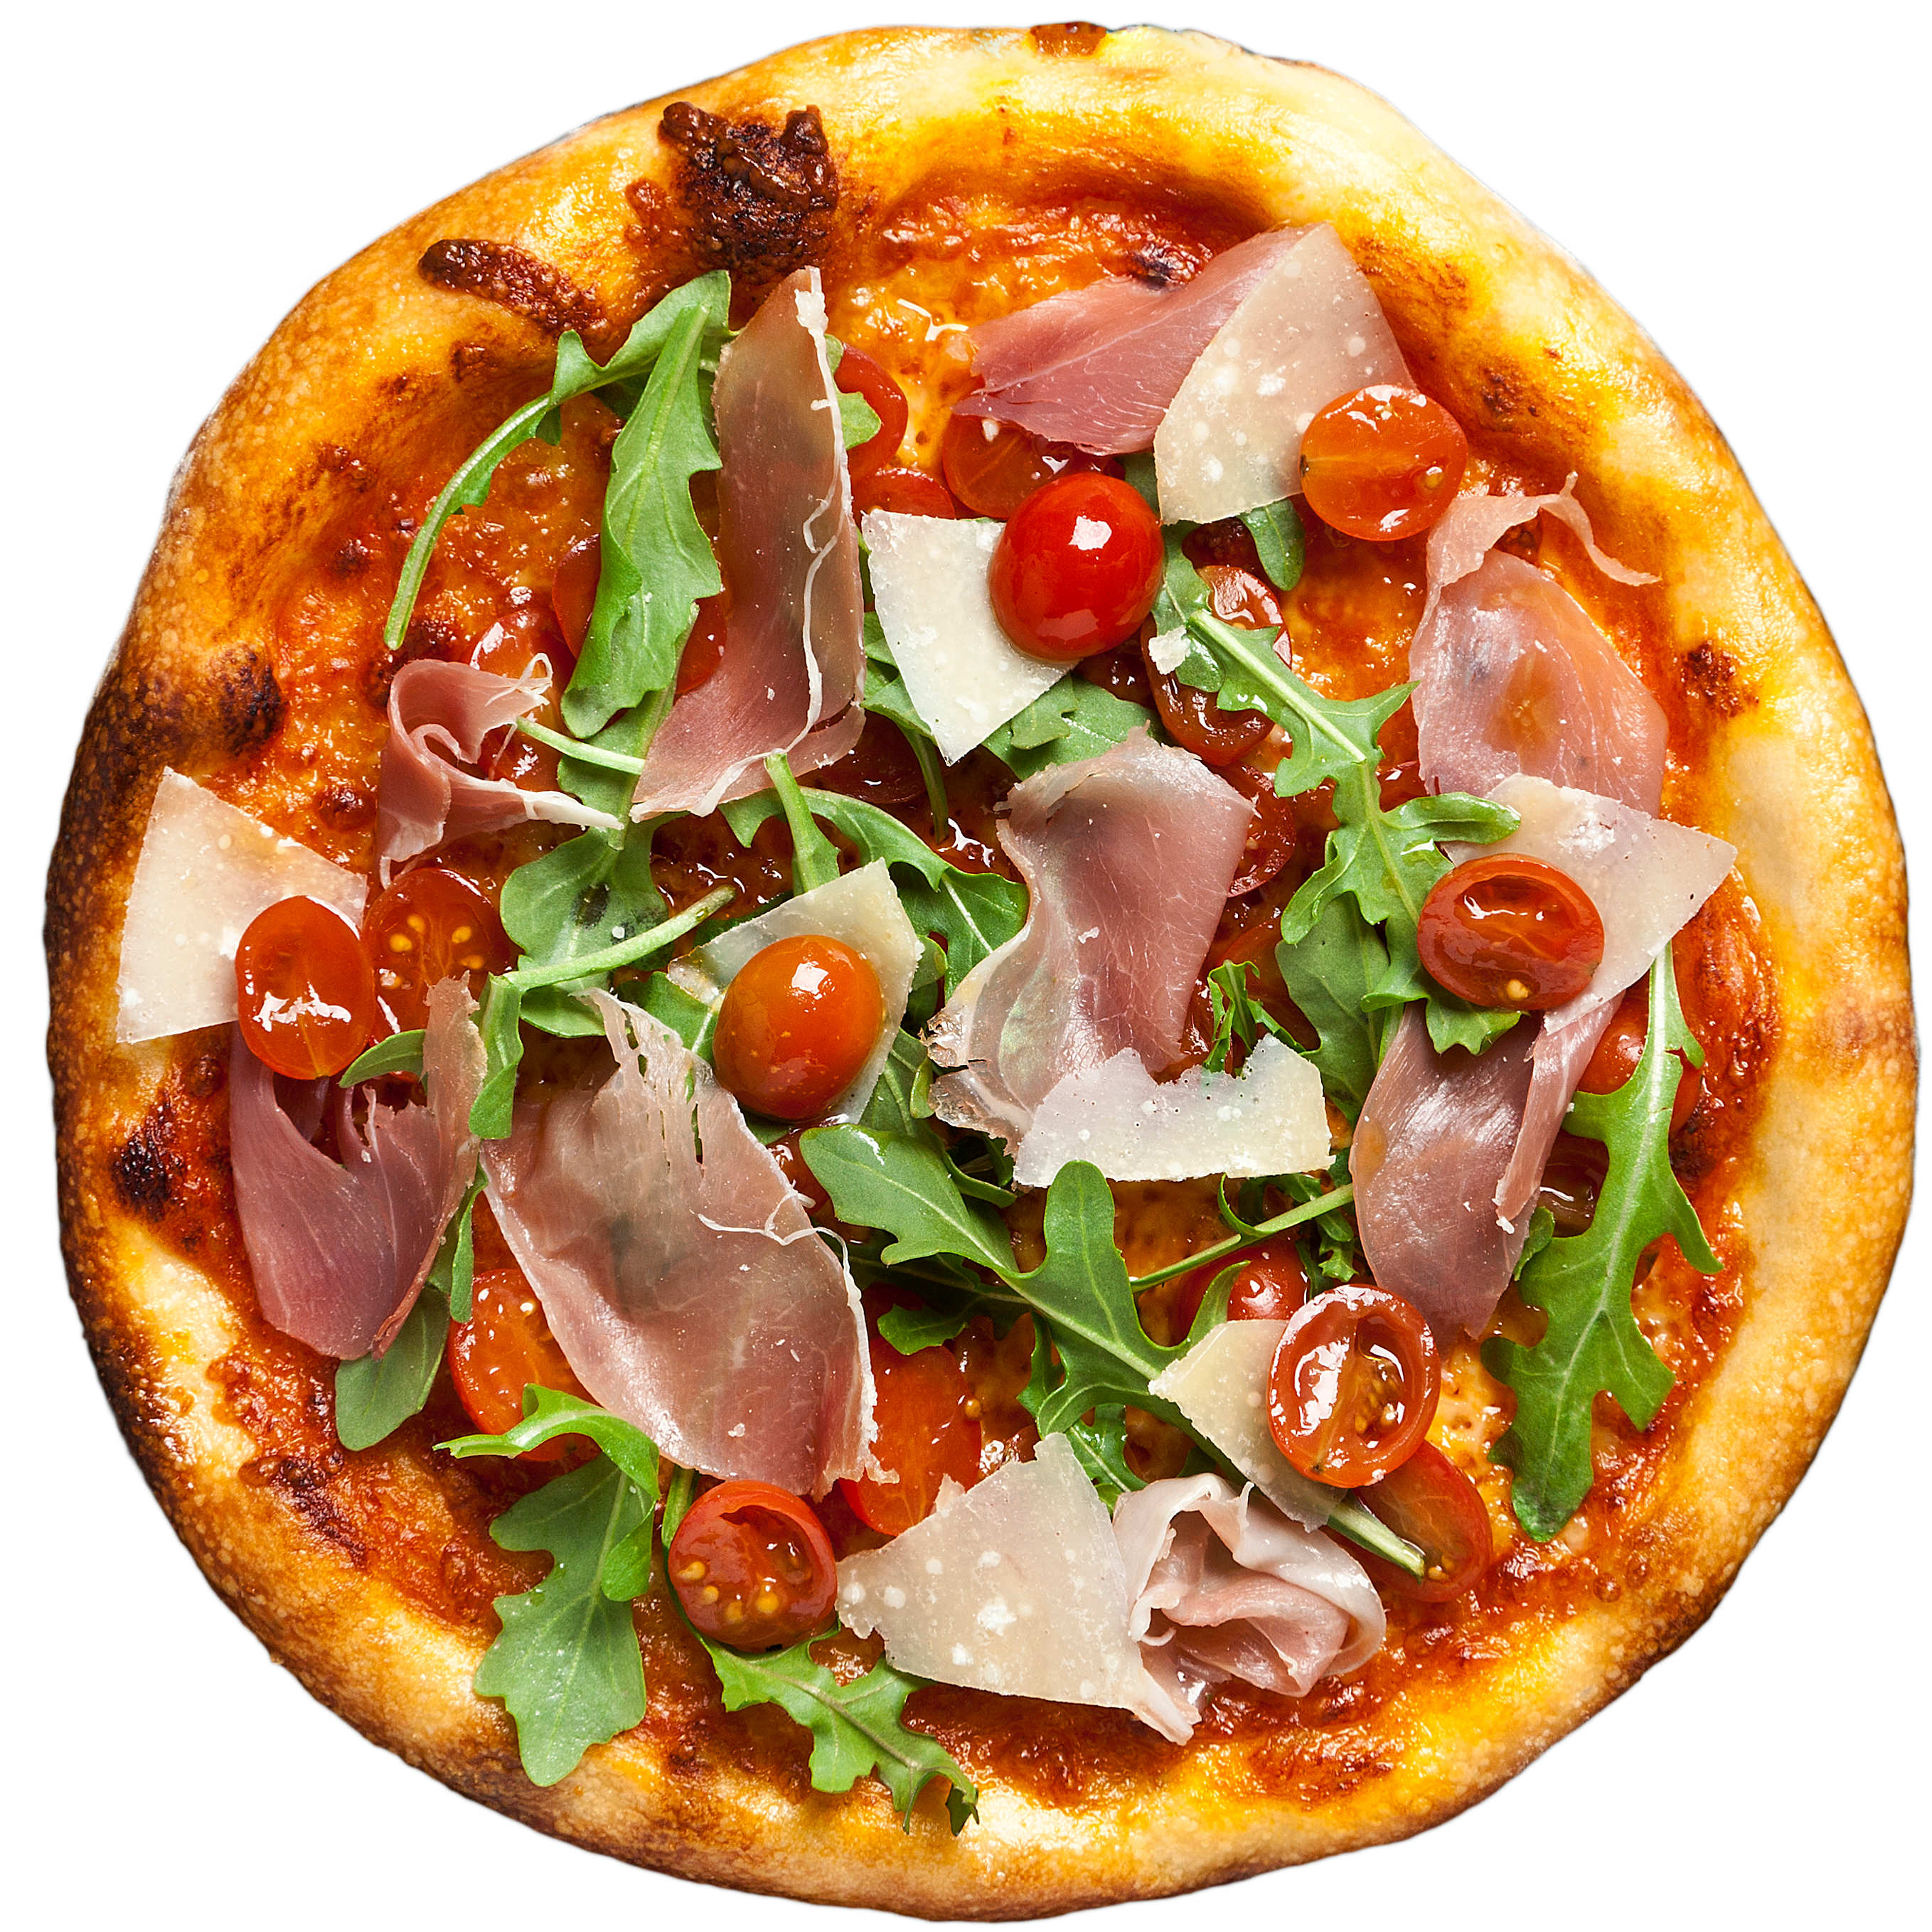
\includegraphics[width=2.5in]{img/example.png}
%	\caption{Picture description.}
%	\label{pic:example}
%\end{figure}

%\subsection{Subsection}
%\lipsum[1]

%\subsection{Subsection}
%\lipsum[1] See Table~\ref{tab:example}.

%\begin{center}
%	\begin{tabular}{| l | l | l |}
%		\hline
%		\bfseries Header 1 & \bfseries Header 2 & \bfseries Header 2 \\
%		\hline
%		Text & text & text \\
%		\hline
%		Text & text & text  \\
%		\hline
%		Text & text & text  \\
%		\hline
%	\end{tabular}
%	\label{tab:example}
%\end{center}

%\lipsum[1] Some references can be found at \footcite{robo4you} or at \footcite{Hope_Learning_TensorFlow}.
%

\filbreak
